\documentclass[internal]{../../../classes/nervtech-research}

\nervsetup{
  company={NervTech},
  project={Node},
  document={Research Notes},
  subtitle={Problem framing, goal association, assumptions and associated research papers},
  docid={NT-N-M-H-000},
  revision={A},
  status={Exploratory Draft},
  author={NervTech Research},
  owner={Robotics Systems Engineering},
  date={2026-07-9},
  stage={Preliminary Research},
  question={Which motor housing architecture will fulfill NT-N-G1, NT-N-G2 and NT-N-G7?},
  keywords={integrated actuator, mechanical design, motor housing, robotics, research notes},
  abstract={This document collates and analyses multiple research papers and notes for fulfilling Node design goals in relation to motor housing design. Its intended purpose is to isolate observations, assumptions, risks, and design direction before committing to a detailed technical design.}
}

\begin{document}
\maketitle
\tableofcontents
\newpage

\section{Research Snapshot}
\researchsnapshot
{Build motor housing to maximise thermal and electromagnetic performance of the actuator, while reducing size and weight.}
{Adhesive bonding is the most suitable mounting method for both stator and rotor, due to its mechanical simplicity, thermal conductivity (scaled by the adhesive chosen) and torque transmissability.
Bearing tolerances should be designed to be of tolerance class P5, to ensure air gap stability and therefore electromagnetic performance.}
{The tolerance stackup of the machined rotor and stator components is uncertain, and must be carefully considered such that the machining processes can achieve the specified air gap tolerance of $\pm$ 0.1175 mm.}
{Do the first iteration of the motor housing design, and do a technical writeup of the design decisions and their impact on the requirements.}

\section{Problem Framing}
\begin{researchquestion}[System Direction]
  What outrunner BLDC motor housing architectures minimises thermal resistance (\textdegree C/W), magnetic flux leakage and Air Gap instability ($\pm$ mm)?
\end{researchquestion}

\section{Preliminary Direction}
This research document will collate results from multiple research papers and notes to inform the design of a motor housing for Node.
The goal is to identify the most promising motor housing architecture that meets the specified design goals (NT-N-G1, NT-N-G2, NT-N-G7).
A preliminary frameless outrunner BLDC motor has been selected, informed by cost and performance requirements.

\section{Assumptions}
\begin{itemize}
  \item The frameless outrunner BLDC architecture will provide the highest torque density and lowest thermal resistance for the Node actuator.
  \item Aluminium provides the best balance of thermal conductivity, weight, and manufacturability for the motor housing.
\end{itemize}

\newpage

\section{Frameless BLDC Architecture}
The selected frameless outrunner BLDC was the SteadyWin WK8115 model with the following dimensions:
\begin{figure}[h!]
  \centering
  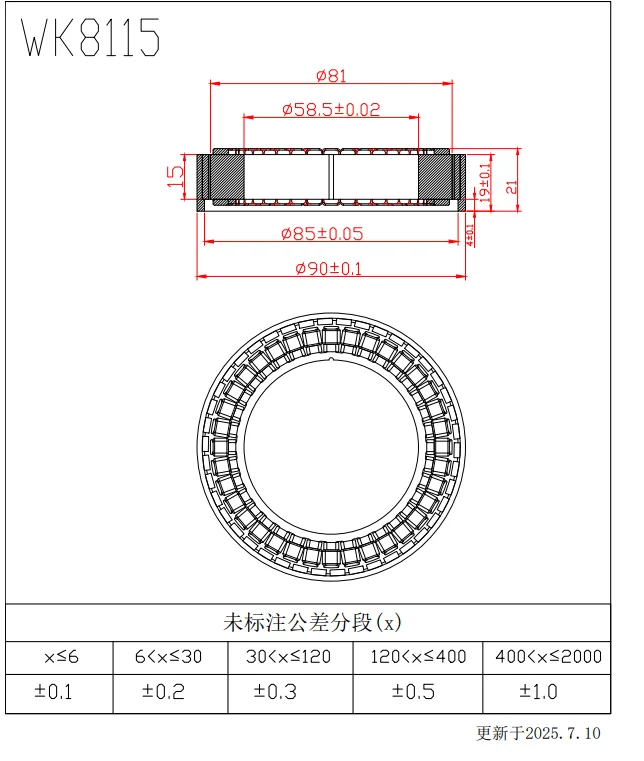
\includegraphics[width=0.8\textwidth]{figures/NT-N-P001.png}
  \caption{SteadyWin WK8115 Dimensions}
  \label{fig:wk8115_dimensions}
\end{figure}
\clearpage
The magnetic, thermal and electrical properties of the motor are taken from the manufacturer as follows:
\begin{figure}[h!]
  \centering
  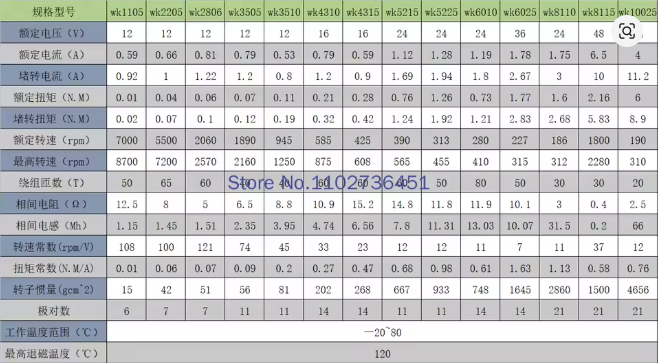
\includegraphics[width=0.8\textwidth]{figures/NT-N-P002.png}
  \caption{SteadyWin WK8115 Specifications}
  \label{fig:wk8115_specifications}
\end{figure}
\newline
Figure~\ref{fig:wk8115_dimensions} will inform the tolerances and mechanical design of the Node motor housing, while Figure~\ref{fig:wk8115_specifications} will inform the thermal and electromagnetic characteristics of the Node actuator.

\section{Existing Motor Integration Guidelines}
Several motion control companies provide mounting and installation guidelines for frameless BLDC motors, which can be applied to the Node motor housing design.
\\\\
\textbf{Note:}
\\
It should be noted that many of these guidelines are for inrunner motors, however the engineering concepts can be transferred between inrunner and outrunner geometries.

\subsubsection{Bearings}
Bearings in the motor housing are critical for maintaining air gap stability and therefore electromagnetic performance \cite{KollmorgenManual}.
Kollmorgen notes that concentricity requirements are noted on the motor datasheet, and should be considered when "sizing and selecting bearings for appropriate radial and preload forces to achieve desired motor running gap clearance and total runout".
While the WK8115 datasheet is vague on concentricity requirements, it does show an air gap of 0.75 mm, and a tolerance stack of $\pm$ 0.07 mm.
\\\\
According to the Maccon Frameless BLDC mounting guide, "the defined manufacturing tolerances in your design should ensure a minimum gap grater
than the half nominal air gap", which is 0.375 mm \cite{MacconManual}.
However, to maximise electromagnetic performance, the air gap should be as consistent as possible, and therefore the concentricity of the bearing stack should be designed to maintain the minimum gap with a factor of safety of 1.5, ensuring a minimum air gap of 0.5625 mm.
This would require the bearing stack to have a minimum tolerance of $\pm$ 0.1175 mm.
According to Maxon, a tolerance class of P5 is recommended for frameless BLDC motors, which is on the scale of micrometers and would therefore be sufficient to maintain the minimum air gap with a factor of safety of 1.5. \cite{MaxonManual}
\\\\
Bearings should also be chosen for the lowest possible friction and high quality lubricant, to reduce motor losses and heat generation.
To do a bearing selection, the expected radial and axial loads on the motor housing must be calculated.
This will be done in the technical design phase; for now, bearings requirements are being defined based on their effect on air gap stability.
\subsubsection{Stator Mounting}
The stator mounting technique is critical for proper thermal management of the motor, and its tolerance will also affect the air gap stability of the motor.
Both Kollmorgen and Maccon note 3 techniques for stator mounting: adhesive bonding, shrink fitting and axial clamping \cite{KollmorgenManual, MacconManual}.
\\\\
\textbf{Axial Clamping}
\\
Securing the stator within 2 "bells", or end caps, puts axial load on the stator and counters torque generated from the rotor via friction.
This is shown for inrunner architectures in the following figures:
\begin{figure}[H]
  \centering
  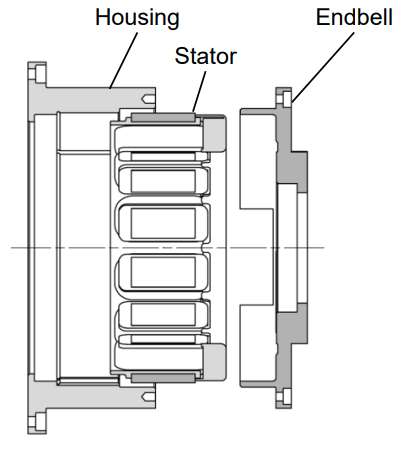
\includegraphics[width=0.4\textwidth]{figures/MabuchiAxialClampingDiagram.png}
  \caption{Axial Clamping of Stator \cite{MabuchiManual}}
  \label{fig:axial_clamping_mabuchi}
\end{figure}
\begin{figure}[H]
  \centering
  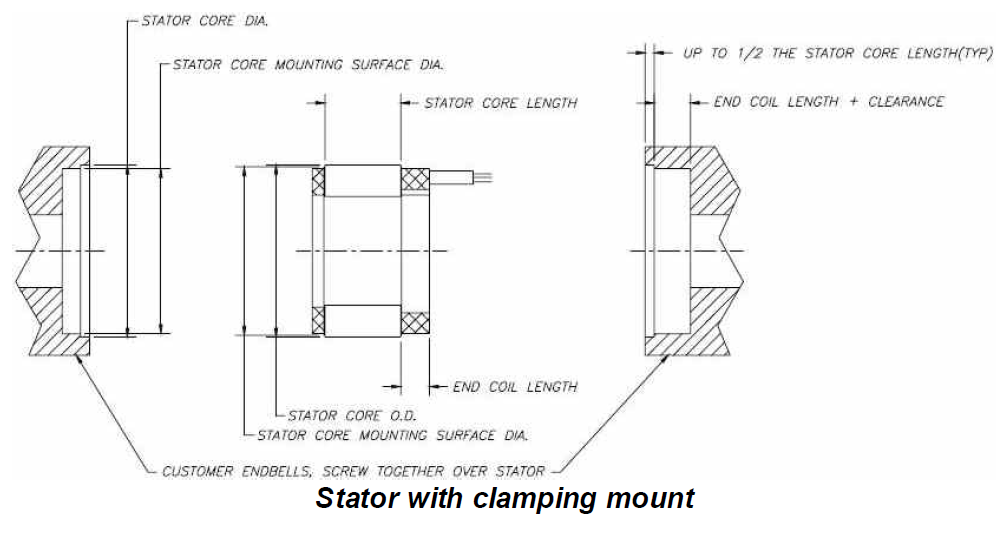
\includegraphics[width=0.8\textwidth]{figures/MacconAxialClampingDiagram.png}
  \caption{Axial Clamping of Stator \cite{MacconManual}}
  \label{fig:axial_clamping_maccon}
\end{figure}

According to Kollmorgen, axial clamping is recommended for "low torque applications" \cite{KollmorgenManual}.
Furthermore, Kollmorgen do not recommended it for "high shock/vibration applications ... or for peak torques greater than 50 N-m without special design considerations".
Geometrically, axial clamping is easier to integrate into housing for inrunner motors vs outrunner motors, making it less suitable for the Node actuator.
Axial clamping also requires a high degree of concentricity between the two end caps, which is difficult to achieve in a small form factor.
\\\\
Since the outrunner stators are located inside the rotor, the end caps would be end caps attached to cylindrical tube-like locating features.
This would reduce the bore diameter of the housing to include machine screws.
This concept is shown in the following figure:
\begin{figure}[H]
  \centering
  
\includegraphics[width=0.6\textwidth]{figures/placeholder.jpg}
  \caption{Axial Clamping of Stator in Outrunner Architecture}
  \label{fig:axial_clamping_outrunner}
\end{figure}
An advantage of axial clamping is high thermal efficiency, as the stator is in direct contact with the end caps, which can be designed to act as heat sinks.
\\\\
\textbf{Shrink Fitting}
\\
Shrink fitting for inrunner motors involved heating the motor housing to expand the bore, and then inserting the stator.
As the housing cools, it contracts and applies a radial load on the stator.
According to Kollmorgen, "aluminium or steel housings may be used effectively to shrink fit stators across a broad peak torque range, generally from <1 N-m up to thousands of N-m" \cite{KollmorgenManual}.
The Mabuchi and Maccon installation guides offer some notes for motor housing design if using shrink fitting.
Mabuchi mention that the housing must meet certain prerequisites for shrink fitting \cite{MabuchiManual}:
\begin{itemize}
  \item "The housing has a thickness that corresponds to the torque" transmitted by the stator.
  \item "The housing has a suitable surface roughness for shrink fit fixing".
\end{itemize}
Maccon also notes that \cite{MacconManual}:
\begin{itemize}
  \item  "Different materials have different thermal expansion coefficients.
  This means that you are limited in the operating/storage temperature when using different materials for stator and housing".
  \item "All mechanical parts have tolerances. When you determine the gap you should always calculate the worst case".
\end{itemize}
Since the procured outrunner motor has a peak transmitted torque of 5.83 N-m, shrink fitting may be an overengineered solution, since it requires consideration of thermal expansion coefficients during operation and stress analysis of the stator to ensure it does not fracture under the radial load.
Furthermore, as will be seen in the next section, adhesive bonding may also provide suitable thermal management if the adhesive is chosen with consideration of its thermal conductivity.
\\\\
\textbf{Adhesive Bonding}
\\
Adhesive bonding is the simplest method of stator mounting, and is suitable for low torque applications.
Kollmorgen notes that "motors in the general peak torque range up to 750 N-m may have the stator bonded in place using a structural epoxy, such as Hysol® EA934NA, 3M™ Scotchweld™ 2214 or other similar adhesives" \cite{KollmorgenManual}.
Adhesive bonding provides the advantage of being easy to implement, however comes at the disadvantage of not having easy disassembly.
\\\\
Kollmorgen, while coming from the perspective of inrunner stators, notes that the stator housing should be designed with "a small shoulder for axial positioning at one end" and that the shoulder "should generally clear the maximum outer diameter of the winding end turn by no less than 1 mm at all circumferential points"" \cite{KollmorgenManual}.
\\\\
For outrunner motor architectures, the stator would be mounted on a cylindrical locating feature, and the shoulder would be a small lip on the cylindrical feature that has the width of the outer laminated edge of the stator and allows enough axial clearance for the winding width.
\\\\
Mabuchi notes that if the temperature rises when curing adhesive bonding, it should not "exceed the heat resistance of the windings" \cite{MabuchiManual}.
This aligns with recommendations from Kollmorgen.
For recommended gaps for proper adhesion, all manuals point to the datasheets of the adhesives.
Kollmorgen notes, as a rule of thumb, that "if using thick structural epoxy, [the] inner diameter of the housing cup should be approximately 0.051 mm - 0.102 mm larger than the maximum outer diameter of the stator", but follows this with pointing to the datasheet of the adhesive for more specific recommendations \cite{KollmorgenManual}.
Small grooves are also recommended as adhesive resorvoirs for structural epoxies, but "are considered optional features per the user's discretion" \cite{KollmorgenManual}.
\\\\
All manuals note that bonding surfaces should be thoroughly cleaned and degreased prior to bonding, to ensure the optimal adhesion.
\\\\
The recommended structural epoxies from the manuals are:
\begin{itemize}
  \item Hysol® EA934NA \cite{KollmorgenManual}
  \item 3M™ Scotchweld™ 2214 \cite{KollmorgenManual}
\end{itemize}

\subsubsection{Rotor Mounting}
\textbf{Axial Alignment Control}
\\
It is noted in the Kollmorgen manual, that the rotor must be properly aligned with the stator to ensure "proper motor performance" \cite{KollmorgenManual}.
Kollmorgen recommends retaining rings installed on shoulders to accomplish this, with the shoulder being on the shaft since this is an inrunner architecture.
For outrunnner architectures, the shoulder would be on the rotor cup, and would locate the rotor relative to the housing bearing using a retaining ring.
The Mabuchi manual also notes that, for their frameless BLDC motors, the stator must cover all magnets on the rotor with an overshoot tolerance of 0.3mm or less \cite{MabuchiManual}.
This should be incorporated into the axial tolerance stack of the rotor, which would include the rotor cup shoulder, the bearing axial play and the stator motor housing.
\\\\
\textbf{Rotor Bonding}
\\
Unlike the stator, the rotor can be bonded to steel rotor cups using retaining compounds \cite{MacconManual} \cite{KollmorgenManual}.
Kollmorgen gives the example of Loctite® 640 retaining compound, and notes they "equire smooth continuous interface diameters and tight fit tolerances" \cite{KollmorgenManual}.
Rotor bonding is likely the most suitable method for the Node actuator, since it is a low torque application and the rotor cup can be designed to have a smooth continuous interface with the rotor.

\subsection{Summary and Comparison Table}


\clearpage

\begin{thebibliography}{9}

\bibitem{KollmorgenManual}
Kollmorgen Corporation (2020) \emph{Mounting and Installation Guidelines for BLDC Motors}, Kollmorgen Technical Documentation.

\bibitem{MacconManual}
Maccon Corporation (2019) \emph{Frameless BLDC Motor Mounting Guide}, Maccon Technical Documentation.

\bibitem{MaxonManual}
Maxon Corporation (2020) \emph{Frameless BLDC Motor Selection Guide}, Maxon Technical Documentation.

\bibitem{MabuchiManual}
Mabuchi Motor Corporation (2018) \emph{BLDC Motor Mounting and Installation Guide}, Mabuchi Technical Documentation.

\end{thebibliography}



\end{document}
